\documentclass[16pt letter]{article}
\title{Implicit Application}
\author{Madiba Hudson-Quansah}
\date{March 2023}
\usepackage{siunitx}
\usepackage{amsmath}
\usepackage{graphicx}
\usepackage{amssymb}
\usepackage{parskip}
\graphicspath{{Graphs/}}
\begin{document}
\maketitle
\pagebreak

\tableofcontents
\pagebreak

\section{}
\label{q:1}

Height of the wall is $y(t)$

Distance from the wall is $x(t)$

From Pythagoras $y(t)^2+x(t)^2 = 10^2$

Known \[\frac{dy}{dx} = 10, \;\; x(t) = 6\]
Unknown \[\frac{dx}{dt}\]

\begin{align*}
	y^2 +x^2 = 10^2                                     \\
	2y \frac{dy}{dt} + 2x \frac{dy}{dt} = 0             \\
	2y(10) + 2x \frac{dy}{dt} = 0                       \\
	20y + 2x \frac{dy}{dt} = 0                          \\
	\frac{dx}{dt} = -\frac{20y}{2x}                     \\
	y^2 = \sqrt{10^2 - x^2}                             \\
	\frac{dx}{dt} = -\frac{20(\sqrt{10^2-(6)^2})}{2(6)} \\
	 & \frac{dx}{dt} = -\frac{40}{3} \; m/sec
\end{align*}
\pagebreak

\section{}
\label{q:2}

\begin{figure}[h]
	\centering
	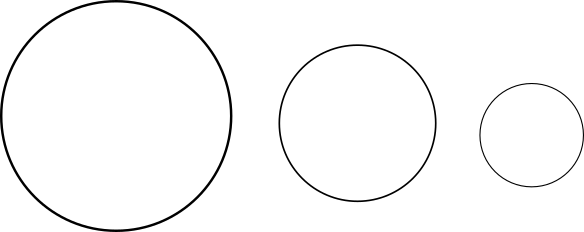
\includegraphics[width=0.55\textwidth]{Application Q2}
	\caption{Balloon deflating}
	\label{fig:deflating}
\end{figure}

Known \[A = 4 \pi r^2, \;\; \frac{dV}{dt} = 2, \;\; r = 12, \;\; V = \frac{4}{3} \pi r^3, \;\;\]
Unknown \[\frac{dr}{dt}\]
\begin{align*}
	4 \pi  r^2 \frac{dr}{dt} = \frac{dV}{dt}        \\
	4 \pi r^2 \frac{dr}{dt} = -2                    \\
	\frac{dr}{dt} = -\frac{2}{4 \pi r^2}            \\[20pt]
	4 \pi r^2 = A                                   \\
	8 \pi  r \frac{dr}{dt} = \frac{dA}{dt}          \\
	8 \pi  r (-\frac{2}{4 \pi r^2}) = \frac{dA}{dt} \\
	 & \frac{dA}{dt} = -\frac{1}{3} ft^2/min
\end{align*}
\pagebreak

\section{}
\label{q:3}

\begin{figure}[h]
	\centering
	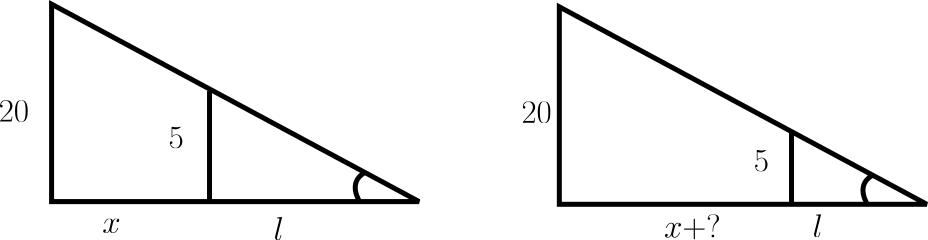
\includegraphics[width=0.80\textwidth]{Application Q3}
\end{figure}

Known \[\frac{dx}{dt} = 4\]
Unknown \[\frac{dl}{dt}\]

\begin{align*}
	\frac{x+l}{20} = \frac{l}{5}                        \\
	x + l = 4l                                          \\
	x = 3l                                              \\
	\frac{x}{3} = l                                     \\
	\frac{dl}{dx} = \frac{1}{3}                         \\[20pt]
	\frac{dl}{dt} = \frac{dl}{dx}  \times \frac{dx}{dt} \\
	\frac{dl}{dt} = \frac{4}{3}                         \\
\end{align*}

\subsection{}

Let $L$ be the sum of the distance from the lamppost and the length of the boy's shadow.
\[\frac{dL}{dt} = \frac{dl}{dt} + \frac{dx}{dt} \therefore \frac{dL}{dt} = \frac{16}{3}\; ft/sec\]

\subsection{}

\[\frac{dl}{dt} = \frac{4}{3}\;ft/sec\]
\pagebreak

\section{}
\label{q:4}

\begin{figure}[h]
	\centering
	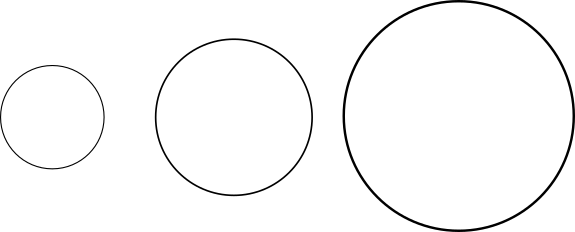
\includegraphics[width=0.55\textwidth]{Application Q4}
	\caption{Balloon inflating}
	\label{fig:inflating}
\end{figure}

Known \[V = \frac{4}{3}\pi r^3, \;\;\ \frac{dV}{dt} = 5\]
Unknown \[\frac{dr}{dt}\]

\begin{align*}
	4 \pi r^2 \frac{dr}{dt} = \frac{dV}{dt}            \\
	4 \pi r^2 \frac{dr}{dt} = 5                        \\
	\frac{dr}{dt} = \frac{5}{4 \pi r^2}                \\[20pt]
	D = r + r \therefore r = 10                        \\[20pt]
	\frac{dr}{dt} = \frac{5}{4 \pi r^2}                \\\
	 & \frac{dr}{dt} = \SI{3.978873577e-3}{ft/\minute}
\end{align*}
\pagebreak

\section{}
\label{q:5}
\begin{figure}[h]
	\centering
	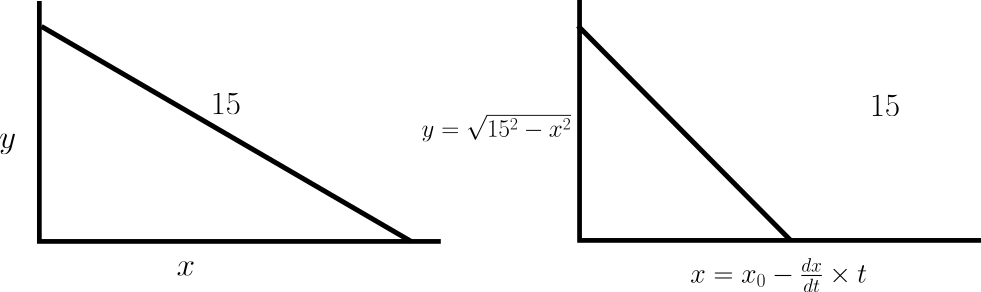
\includegraphics[width=0.80\textwidth]{Application Q5}
\end{figure}

Known
\begin{align*}
	\frac{dx}{dt} = \frac{1}{4}               \\
	\text{When } t = 0, \; x = 10             \\
	\therefore t = 0, \; y = \sqrt{15^2-10^2} \\
	y = 5\sqrt{5}
\end{align*}

\begin{align*}
	y^2 +x^2 = 15^2                                                                           \\
	2y\frac{dy}{dt} + 2x \frac{dx}{dt} = 0                                                    \\
	\frac{dy}{dt} = \frac{-2x(-\frac{1}{4})}{2y}                                              \\
	\frac{dy}{dt} = \frac{\frac{1}{2}x}{2y}                                                   \\[20pt]
	x(t) = x(0) + \frac{dx}{dt}  \times t                                                     \\
	x(t) = 10 - \frac{1}{4}  \times  t                                                        \\
	x(t) = 10 - \frac{t}{4}                                                                   \\
	y(t) = \sqrt{15^2-x^2}                                                                    \\[20pt]
	x = 10 - \frac{t}{4}, \;\; t = 12, \;\; y = \sqrt{15^2-x^2}                               \\
	\frac{dy}{dt} = \frac{\frac{1}{2}(10 - \frac{t}{4})}{2(\sqrt{15^2-(10 - \frac{t}{4})^2})} \\
	 & \frac{dy}{dt}  = 0.132\; ft/sec
\end{align*}


\section{}
\label{q:6}

\begin{figure}[h]
	\centering
	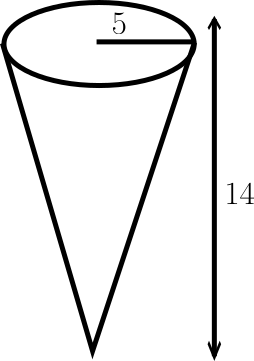
\includegraphics[width=0.20\textwidth]{Application Q6 A}
\end{figure}
Known \[\frac{dV}{dt} = -2, \;\; r= 5,\;\; h=14,\;\; V= \pi r^2 \frac{h}{3}\]
Unknown \[ \frac{dh}{dt},\;\; \frac{dr}{dt}\]

\begin{align*}
	\frac{dV}{dt} = (\pi r^2)(\frac{1}{3}\frac{dh}{dt}) + (2 \pi r \frac{dr}{dt})(\frac{h}{3}) \\
	\frac{dV}{dt} = \frac{\pi r^2}{3} \frac{dh}{dt} + \frac{2 \pi rh}{3}\frac{dr}{dt}
\end{align*}

\begin{figure}[h]
	\centering
	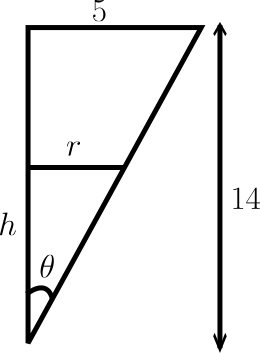
\includegraphics[width=0.20\textwidth]{Application Q6 B}
\end{figure}
\begin{align*}
	\frac{r}{h} = \frac{5}{14}                 \\
	r = \frac{5}{15}h                          \\[10pt]
	h = 6                                      \\
	r = \frac{5(6)}{14}                        \\
	r = \frac{15}{7}                           \\[20pt]
	\frac{dr}{dt} = \frac{5}{14} \frac{dh}{dt} \\
\end{align*}
\subsection{}
\begin{align*}
	-2 = \frac{\pi (\frac{15}{7})^2}{3}\frac{dh}{dt} + \frac{2 \pi (\frac{15}{7})(6)}{3}(\frac{5}{14})\frac{dh}{dt} \\
	-2 = \frac{75}{49}\pi \frac{dh}{dt} + \frac{150}{49}\pi \frac{dh}{dt}                                           \\
	-2 = \frac{225}{49}\pi \frac{dh}{dt}                                                                            \\
	- \frac{2}{\frac{225}{49}\pi} = \frac{dh}{dt}                                                                   \\
	 & \frac{dh}{dt} = -\frac{98}{225}\;ft/hour
\end{align*}

\subsection{}
\begin{align*}
	\frac{dh}{dt} = -\frac{98}{225} \;\; \text{when } h = 6 \\
	\frac{dr}{dt} = \frac{5}{14}(-\frac{98}{225}\pi )       \\
	 & \frac{dr}{dt} = -\frac{7}{45}\pi\; ft/hour
\end{align*}
\pagebreak

\section{}
\label{q:7}

\begin{figure}[h]
	\centering
	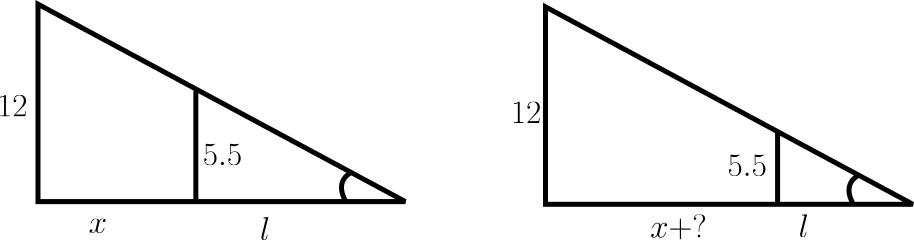
\includegraphics[width=0.90\textwidth]{Application Q7}
\end{figure}

Known \[\frac{dx}{dt} = 2\]
Unknown
\begin{gather*}
	\text{Let } L = x + l\\
	\frac{dL}{dt} \text{ when } x= 25
\end{gather*}

\begin{align*}
	\frac{x+l}{12} = \frac{l}{5.5}                \\
	x+l = \frac{24}{11}l                          \\
	x = \frac{13}{11}l                            \\
	 & \frac{11}{13}x = l                         \\
	 & \frac{11}{13}\frac{dx}{dt} = \frac{dl}{dt}
\end{align*}

\subsection{}

\begin{align*}
	L = x +l
	L = x + \frac{11}{13}x                     \\
	L = \frac{24}{13}x                         \\
	\frac{dL}{dt} = \frac{24}{13}\frac{dx}{dt} \\
	 & \frac{dL}{dt} = \frac{48}{13} \;ft/sec
\end{align*}
\pagebreak

\section{} % (fold)
\label{q:8}
\begin{figure}[h]
	\centering
	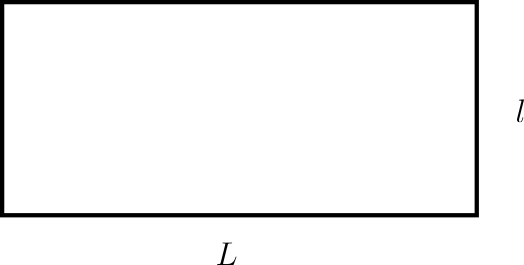
\includegraphics[width=0.55\textwidth]{Application Q8}
\end{figure}

Known \[L = 3l, \;\; \frac{dl}{dt} = -2\]
Unknown \[\frac{dL}{dt}\]

\subsection{}
\begin{align*}
	\frac{dL}{dt} = 3\frac{dl}{dt}   \\
	\frac{dL}{dt} = -6 \; inches/min \\
\end{align*}

\subsection{}
Known \[A = L  \times l, \;\; \frac{dl}{dt} = -2,\;\; l = 6\]
\begin{align*}
	\frac{dA}{dt} = (L)(\frac{dl}{dt}) + (\frac{dL}{dt})(l) \\
	\frac{dA}{dt} = 3(6)(-2) + 3(-2)(6)                     \\
	 & \frac{dA}{dt} = -72 \; inches^2/min
\end{align*}
\pagebreak

\section{}
\label{q:9}
\begin{figure}[h]
	\centering
	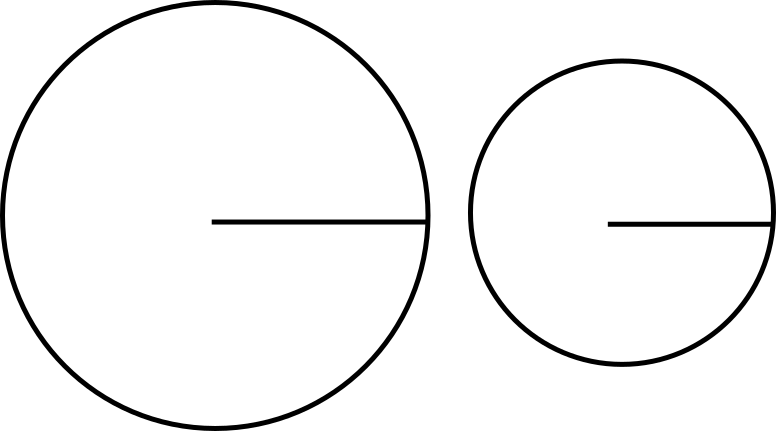
\includegraphics[width=0.45\textwidth]{Application Q9}
\end{figure}
Known \[\frac{dA}{dt} = -0.5, \;\; A = 12\]
Unknown \[\frac{dr}{dt}\]

\begin{align*}
	A = \pi r^2                                                 \\
	12 = \pi r^2                                                \\
	\frac{12}{\pi } = r^2                                       \\
	\sqrt{\frac{12}{\pi }} = r                                  \\[20pt]
	\frac{dA}{dt} = 2 \pi r \frac{dr}{dt}                       \\
	-0.5 = 2 \pi (\sqrt{\frac{12}{\pi }})\frac{dr}{dt}          \\
	\frac{-0.5}{2 \pi (\sqrt{\frac{12}{\pi }})} = \frac{dr}{dt} \\
	 & \frac{dr}{dt} = -0.0407\; m/sec
\end{align*}
\pagebreak

\section{}
\label{q:10}
\begin{figure}[h]
	\centering
	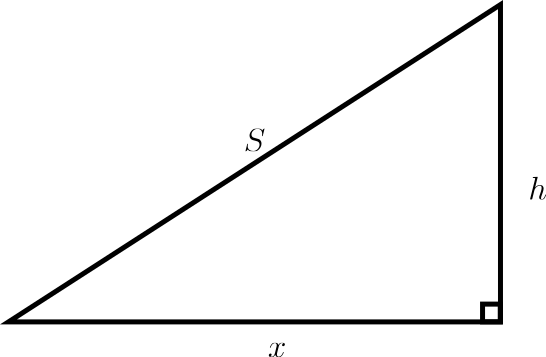
\includegraphics[width=0.55\textwidth]{Application Q10}
\end{figure}
Known \[\frac{dh}{dt} = 15\]

\subsection{}
\begin{align*}
	350^2 + h^2 = S^2                                 \\
	0 + 2h \frac{dh}{dt} = 2S \frac{dS}{dt}           \\[20pt]
	h = h_0 + \frac{dh}{dt}  \times t                 \\
	h = 0 + 15  \times  (20)                          \\
	h = 300                                           \\[20pt]
	350^2 + 300^2 = S^2                               \\
	212500 = S^2                                      \\
	50\sqrt{85} = S                                   \\
	2(300)(15) = 2(50\sqrt{85}) \frac{dS}{dt}         \\
	\frac{2(300(15))}{2(50\sqrt{85})} = \frac{dS}{dt} \\
	 & \frac{dS}{dt} = 9.762\;ft/sec
\end{align*}

\subsection{}
\begin{align*}
	h = 15  \times  6                          \\
	h = 900                                    \\[20pt]
	350^2 + 900^2 = S^2                        \\
	50\sqrt{373} = S                           \\
	2(900)(15) = 2(50\sqrt{373}) \frac{dS}{dt} \\
	 & \frac{dS}{dt} = 13.980\; ft/sec
\end{align*}

\end{document}
